\chapter{Coupling of $p_y$ Modes and the Invisibility Angle \label{cap:invisibility}}
In electrostatics, dipolar interactions can be described using second-order Legendre polynomials, particularly with $P_2(\cos(\theta))=3\cos^2(\theta)-1$, where $\theta$ epresents the angle between two electric dipoles. The angular value $\theta_m
\approx 0.62$ radians is known as the \textit{magic angle}, as it cancels the dominant dipolar interaction term \citep{medmagic}.

This chapter focuses on the experimental study of vertical dipolar modes, also referred to as $p_y$modes, whose existence requires surpassing the cutoff condition: a sufficiently short wavelength, combined with an index contrast $\Delta n$and an appropriate transverse dimension. These modes exhibit a transverse distribution characterized by two symmetric lobes relative to the horizontal axis and a phase difference of $\pi$ between them.

\section{Couplers}

When studying the evanescent coupling between $p_y$ modes in elliptical waveguides, two limiting configurations are distinguished: when the waveguides are arranged horizontally (aligned along the $x$-axis), the coupling—denoted $\varkappa_\pi$​—is positive; conversely, for vertical couplers (aligned along $y$), the coupling $\varkappa_\sigma$ eis negative \citep{Pmodecoupling}. This sign change is interpreted as an interference effect between the lobes of the $p_y$mode, whose lobular profile with odd symmetry about the horizontal axis generates different coupling conditions depending on the relative orientation of the waveguides.

This behavior presents an analogy\footnote{This analogy is purely geometric and modal. It does not imply the existence of electron clouds, interatomic potentials, or bonding energy in the chemical sense. However, it is retained as a useful conceptual tool to describe the relative orientation of the modes and the effect of symmetry on the strength and sign of the coupling. Its utility lies in the clarity with which it communicates differences in the nature of coupling, especially in multi-orbital systems like those studied in this thesis.} with the $\sigma$ and 
$\pi$ chemical bonds formed in carbon chains: in quantum chemistry, $\sigma$ bonds correspond to frontal (axial) overlaps of orbitals, while $\pi$ bonds arise from lateral overlaps, typically between $p$ corbitals with nodes along the bonding axis. Analogously, we refer here to \textit{coupling} $\varkappa_\sigma$ as that which occurs through axial superposition between modes with suitable symmetry, generating a profile without a transverse node; whereas \textit{coupling} $\varkappa_{\pi}$ or $\varkappa_{\theta = 0}$ corresponds to a lateral superposition, in which the modal distribution exhibits a central node.

To verify this effect, 20 dimers were experimentally fabricated with a fixed separation of 25 $\mu$m and a propagation length of 15 mm, varying the angle between waveguides from 0.00 rad to 1.57 rad. The initial excitation was generated using a spatial light modulator (SLM), programmed to selectively couple the $p_y$ mode into one of the waveguides.

\begin{figure}[H]
	\centering
	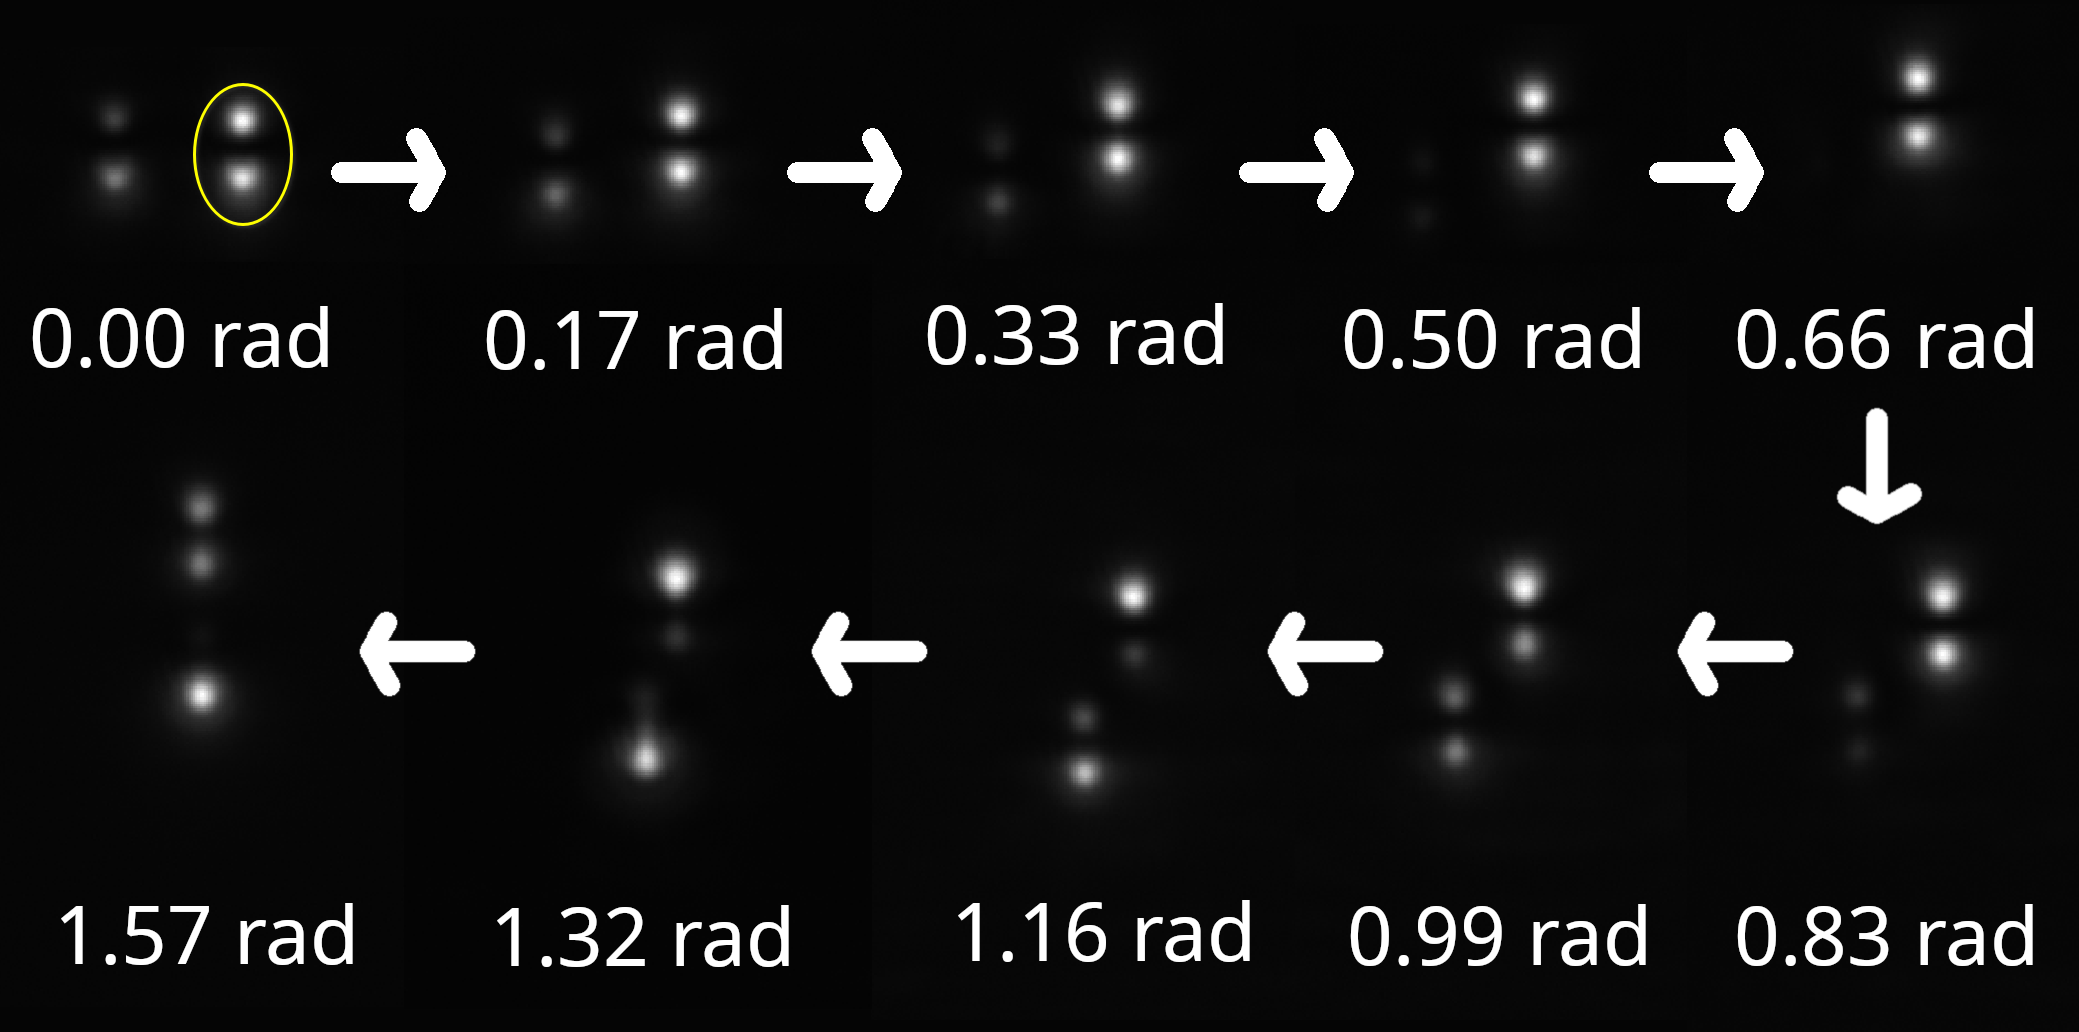
\includegraphics[width=0.7\linewidth]{media/26um_15mm_angles_v2.png}
\caption[Experimental angular sweep]{Experimental angular sweep for a propagation distance of 15 mm. The effect of the magic angle is observed between 0.50 and 0.66 rad. \label{fig:angulobarrido}}
\end{figure}

The obtained images were analyzed following the procedure described in Section~\ref{sec:imageanal}. Subsequently, using equation (\ref{eqn:coupling-simp}), which describes the dynamic coupling, the effective coupling was quantitatively characterized as a function of the angle $\theta$, measured from the horizontal. To correctly reflect the continuity of the coupling with the angle, the sign of the coupling was adjusted in the theoretical fit, as shown in Figure~\ref{fig:invisibility-coup}.
\begin{figure}[H]
    \centering
    
\includegraphics[width=0.6\linewidth]{codigo/eigenvalues_vs_angle.png}
   \caption[Propagation constants and angular couplings for P modes]{Propagation constants and couplings as a function of the angle for $p_y$modes, numerically calculated using EME. The results are compared with experimental data extracted from Figure \ref{fig:angulobarrido}. \label{fig:invisibility-coup}}
\end{figure} \vspace{-2ex}
\section{Honeycomb Lattices}
The honeycomb lattice, known for being the underlying crystalline structure of graphene, presents properties relevant to this thesis, particularly in its Bloch bands: both are dispersive and exhibit a Dirac point \citep{honeycombdirac}. Once the fabrication parameters from the previous section were determined, the same effect was studied in a honeycomb lattice by keeping the distance between sites constant while varying the angle (Figure \ref{fig:HCLBW}).

\begin{figure}[H]
	\centering
	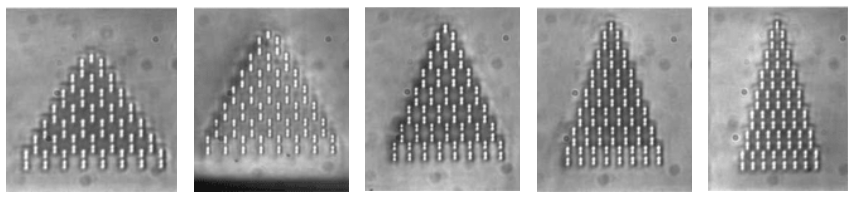
\includegraphics[width=\linewidth]{media/honeycomb_lattices_bw.png}
	\caption[Microscope images of honeycomb-type photonic lattices for P modes]{Microscope images of honeycomb-type photonic lattices for $p_y$ modes under white light illumination. \label{fig:HCLBW}}
\end{figure} \vspace{-3ex} A first-neighbors model would only consider the vertical coupling $\varkappa_\sigma$ and the angular coupling $\varkappa_\theta$. However, an accurate description of the experimental data requires including couplings up to third neighbors, as well as non-orthogonality corrections. Figure~\ref{fig:honeycombmodel} shows a schematic of the complete model. The system's Hamiltonian is expressed as:
\begin{equation}
	\hat{H}_\Sigma = \hat{H}_{NN} + \hat{H}_{NNN} + \hat{H}_{NNNN},
\end{equation}
where $\hat{H}_{NN}$, $\hat{H}_{NNN}$ and $\hat{H}_{NNNN}$ contain the couplings to first neighbors ($\varkappa_\sigma$ y $\varkappa_\theta$), second neighbors ($t_\pi$ and $t_{\theta 2}$), and third neighbors ($t_{\theta 1}$ y $t_{\theta 3}$), respectively (see Figure \ref{fig:honeycombmodel}).

\begin{figure}[H]
	\centering
	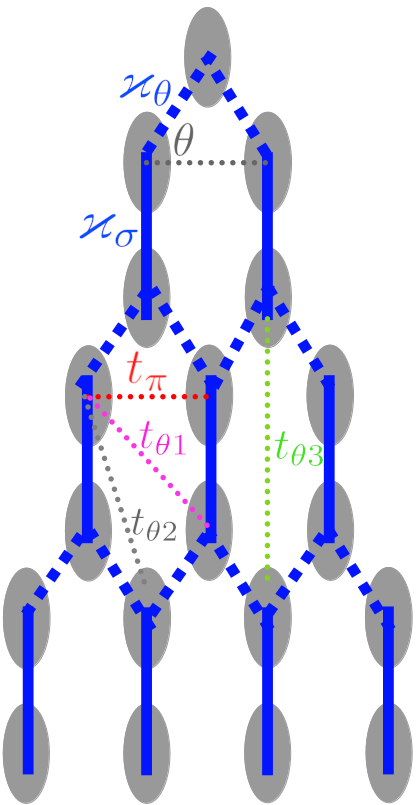
\includegraphics[width=0.25\linewidth]{media/honeycomb-lattice.png}
	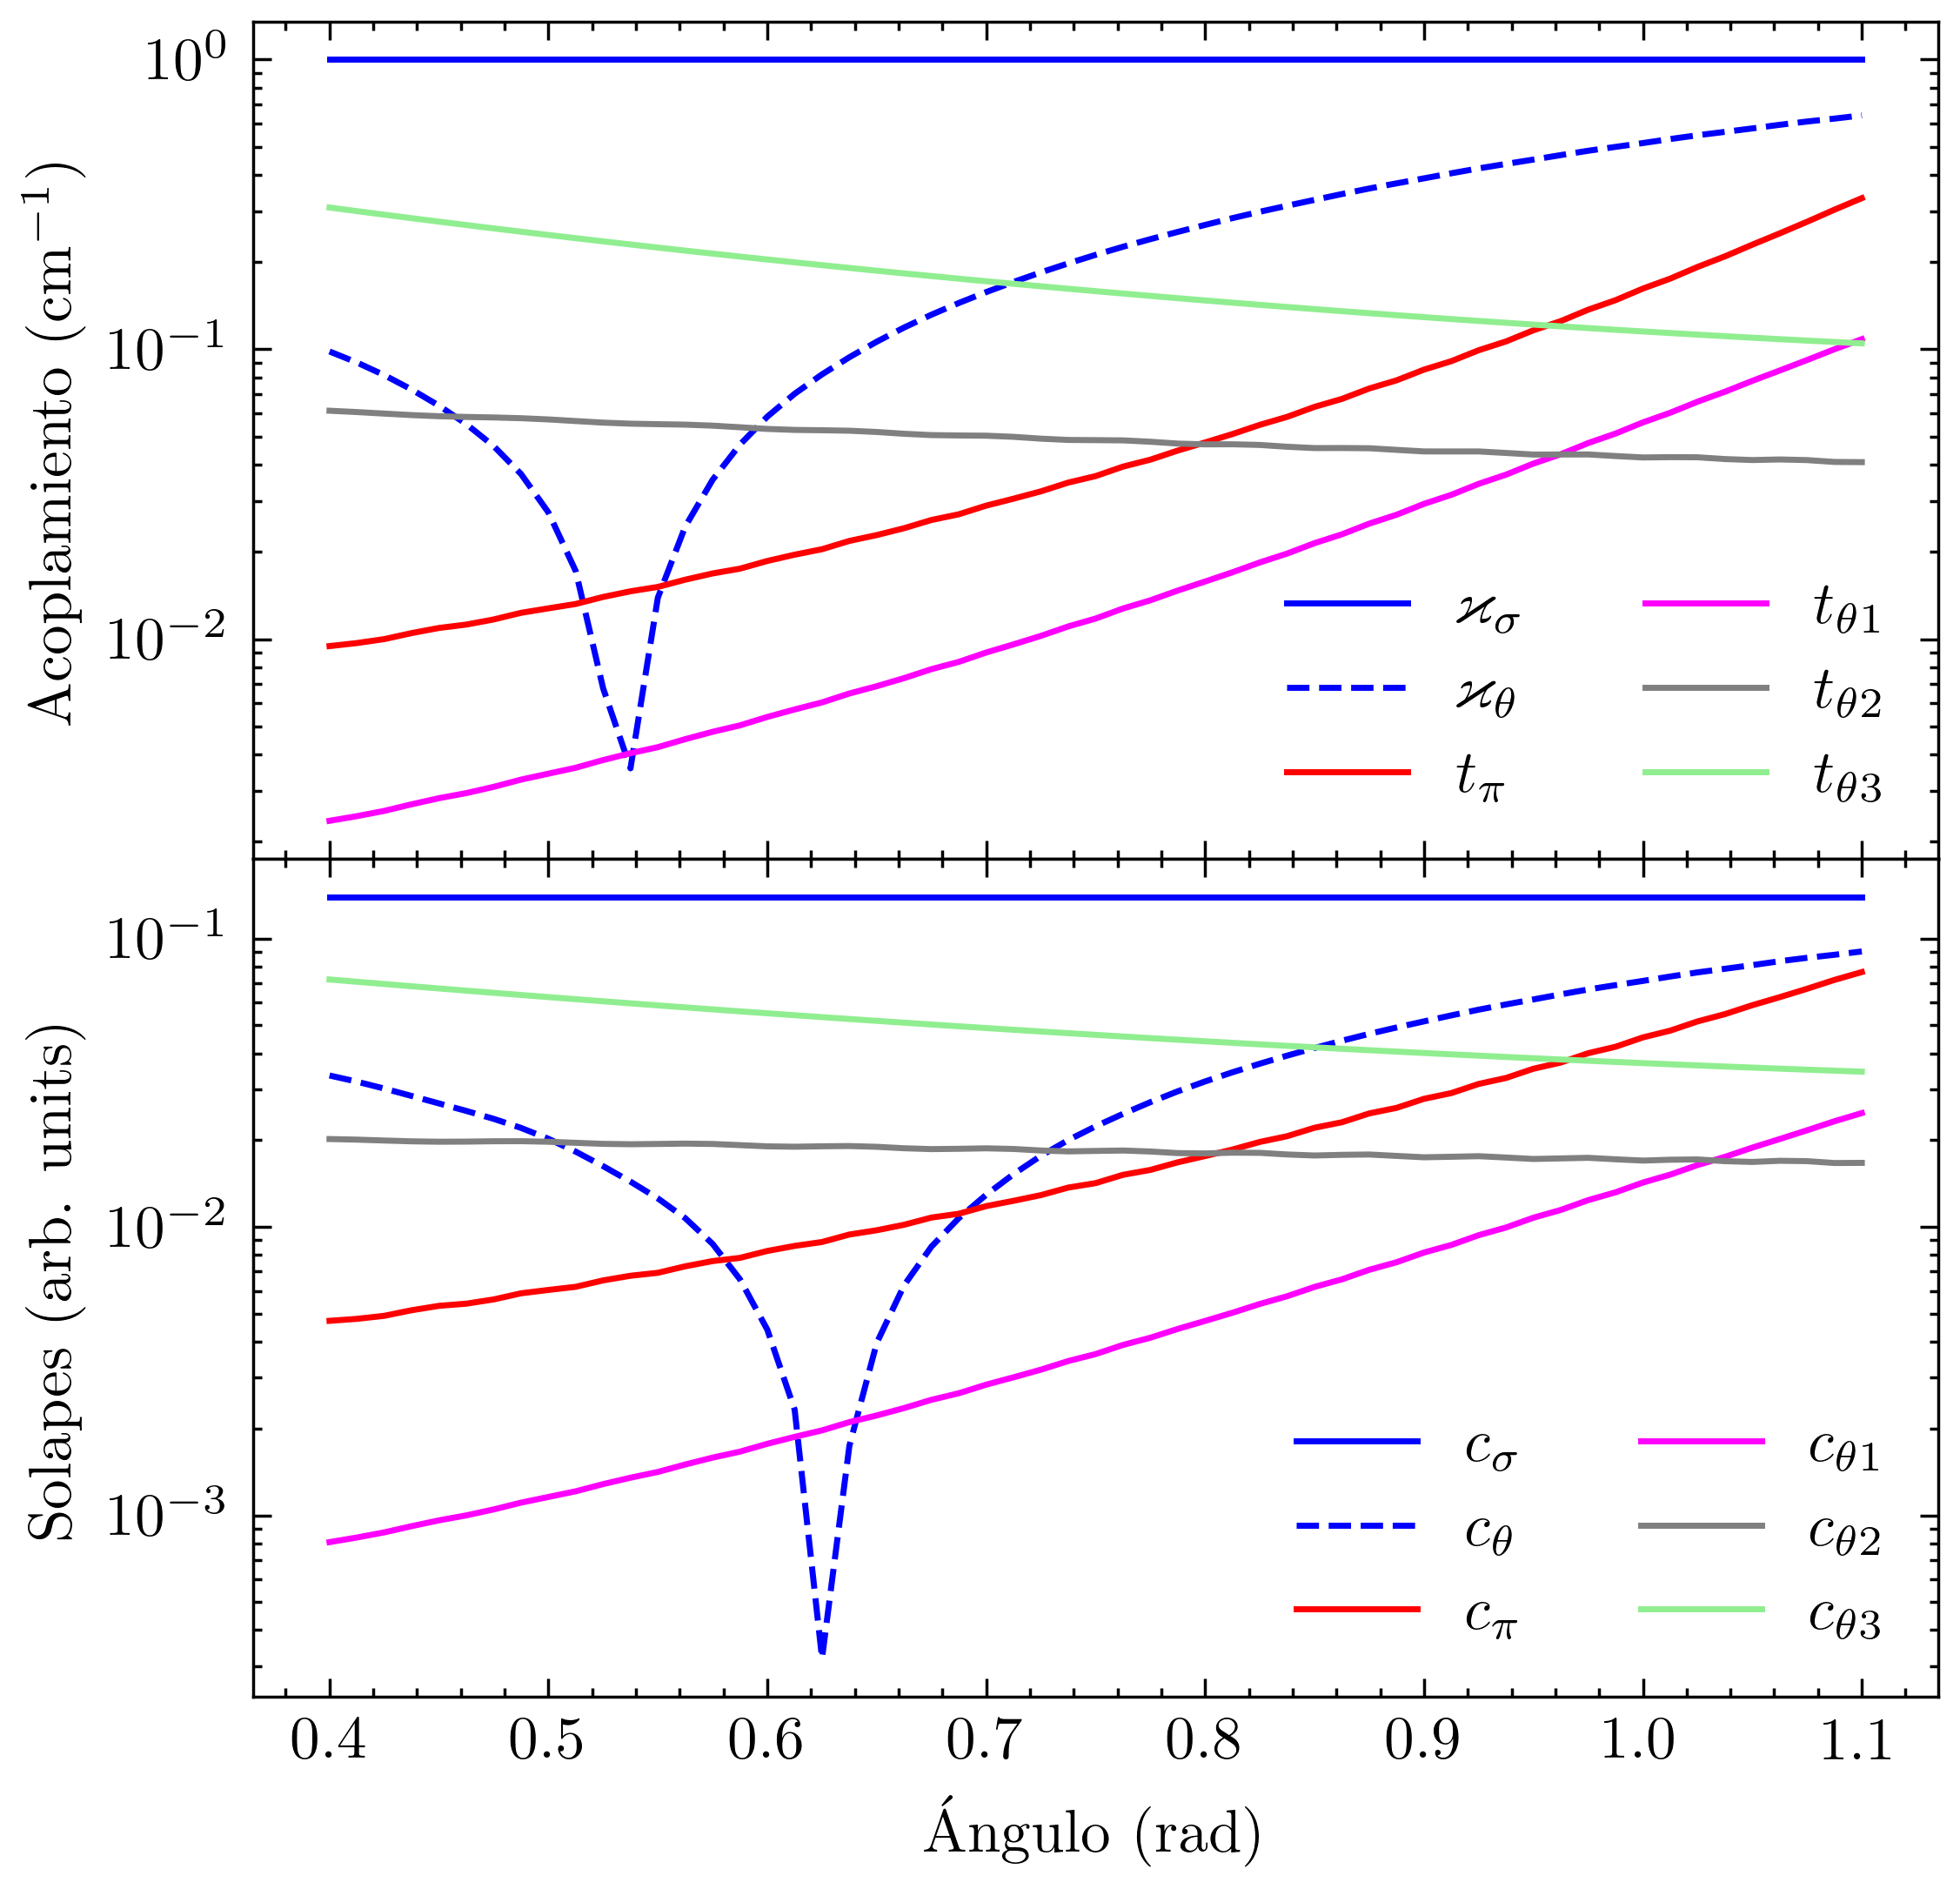
\includegraphics[width=0.55\linewidth]{codigo/NNNN_overlap_vs_angle.png}
	\caption[Honeycomb model for $p_y$ modes with couplings up to third neighbors]{\textbf{Left:} Schematic of the honeycomb model for $p_y$ modes with couplings up to third neighbors. \textbf{Right:} (Top) Absolute values of the couplings as a function of the angle $\theta$. (Bottom) Normalized overlap integrals as a function of the angle $\theta$.\label{fig:honeycombmodel}}
\end{figure} \vspace{-3ex} Furthermore, the non-orthogonal matrix $\hat{c}$ is defined from the matrix $\hat{P}$ [equation~(\ref{eqn:CMTnum})] as $c_{ij} = P_{ij}/I$, where $I = P_{ii}$ is the intensity of the $p_y$ mode, so that the diagonal elements of $\hat{c}$ are equal to 1. Similarly to the couplings, Figure \ref{fig:honeycombmodel} plots the magnitude of the overlaps $c_{ij}$ eas a function of the angle.
The non-Hermitian Hamiltonian $\hat{H}_\Sigma' \equiv \hat{c}^{-1} \hat{H}_\Sigma$ describes the dynamics of the lattice and incorporates both non-orthogonal effects and long-range couplings. Figure \ref{fig:honeycomb-spectra} shows the spectrum as a function of the angle $\theta$. Two main regions are distinguished: one for angles $0.4 < \theta < 0.7$, where the eigenvalues cluster into three quasi-flat bands, and another for angles $0.7 < \theta < 1.1$, where the gap decreases in magnitude, thus increasing transport in the lattice. The inverse participation ratio (IPR) of each eigenstate is calculated as $\text{IPR} = \sum_i I_i^2/(\sum_i I_i)^2$. This allows for an adequate description of the experimental data shown in the right panel of Figure \ref{fig:honeycomb-spectra}.
\begin{figure}[H]
	\centering
	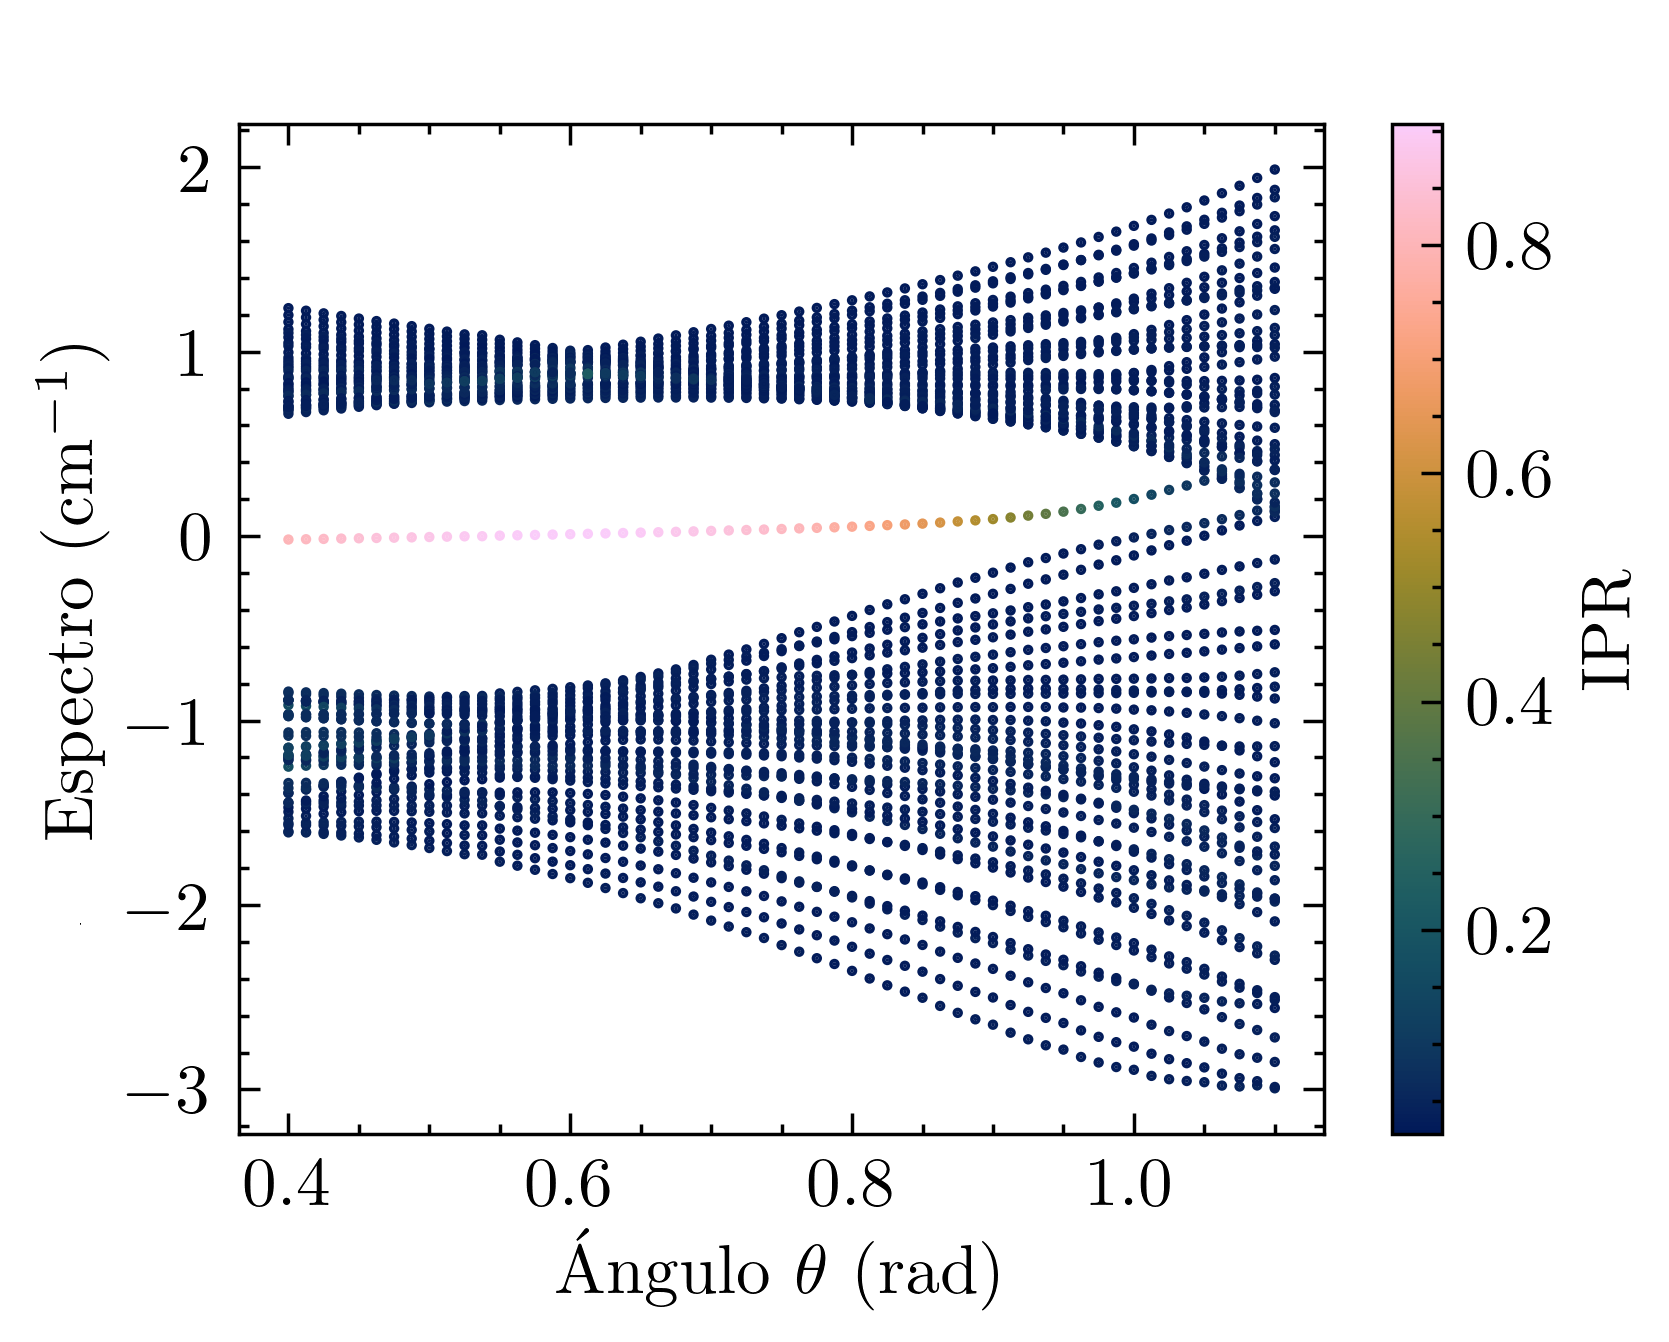
\includegraphics[width=0.45\linewidth]{codigo/honeycomb_eigenvalues_vs_angle.png}
	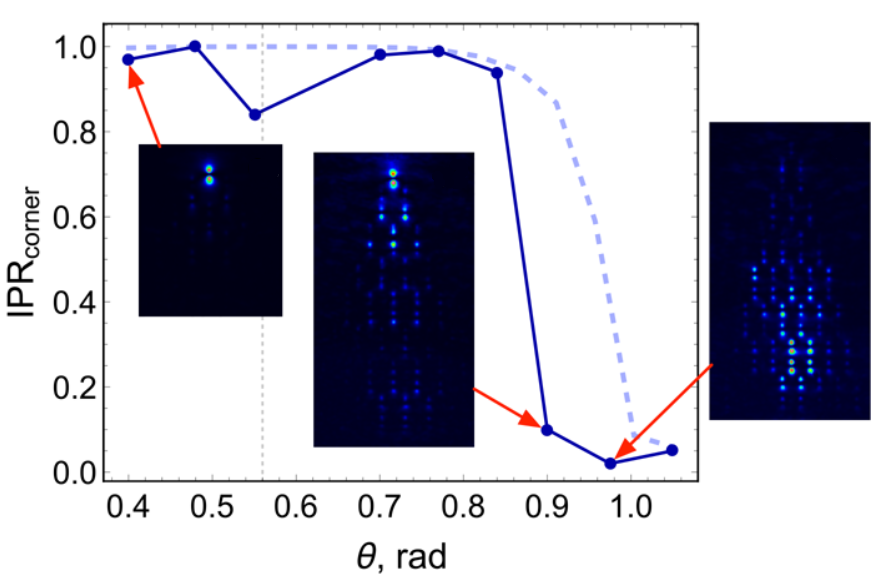
\includegraphics[width=0.5\linewidth]{media/ipr-corner-exp.png}
	\caption[Spectrum of the honeycomb lattice of $p_y$ modes as a function of the angle]{\textbf{Left:} Spectrum of the matrix $\hat{H}_\Sigma'$ as a function of the angle. Each point is colored according to its inverse participation ratio (IPR). \textbf{Right:} Inverse participation ratio for the corner site excitation as a function of the angle $\theta$.\label{fig:honeycomb-spectra}}
\end{figure} \vspace{-3ex}
The strong localization observed when exciting the corner site is explained by the fact that the projection of the initial condition onto the eigenstates corresponds predominantly to the eigenstate with a null eigenvalue. The existence of this eigenstate is due to the topology exhibited by the Hamiltonian $\hat{H}_\Sigma'$ in reciprocal or Bloch space. Although it is possible to calculate the bulk polarization using Wilson loops and determine that its value is discretized as $\mathbf{P} = (0.5, 0.5)$, it is more illustrative to note that the lattice can be decomposed into quasi-SSH chains (see Figure \ref{fig:quasi-ssh}). In both schemes, quantization is a consequence of the inversion symmetry present in the lattice.
\begin{figure}[H]
	\centering
	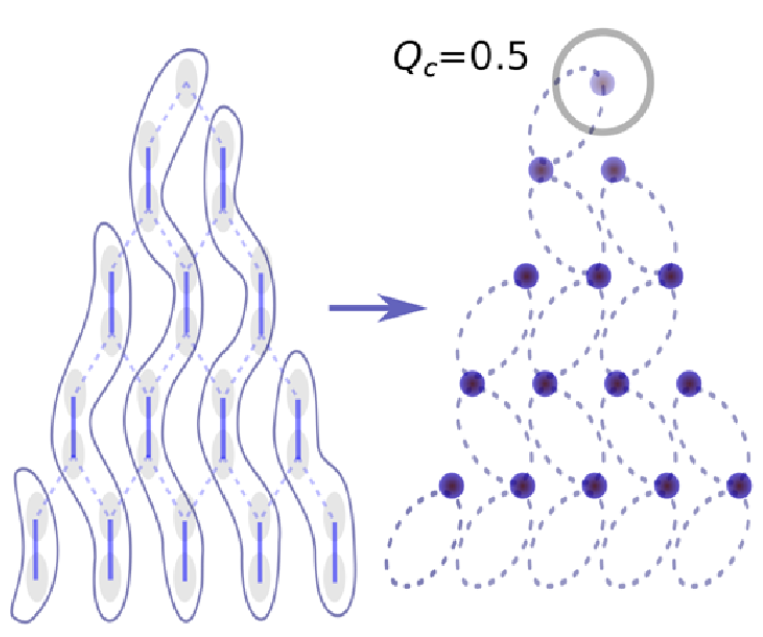
\includegraphics[width=0.40\linewidth]{media/cuasi-ssh.png}
	\hfill
	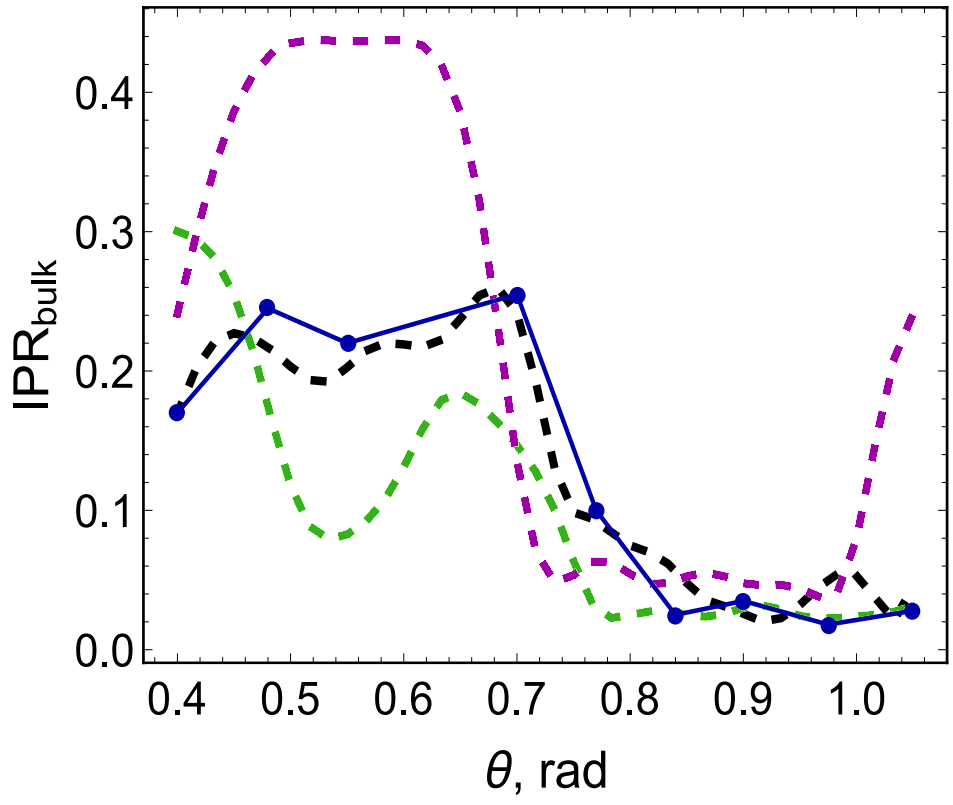
\includegraphics[width=0.40\linewidth]{media/ipr-bulk-exp.png}
	\caption[Decomposition of the lattice into quasi-SSH chains]{
		\textbf{Left: }
		Decomposition of the lattice in the flat-band limit into isolated dimer SSH chains. \textbf{Right: } IPR for the experimental excitation of the central site of the lattice (points connected with lines to guide the eye) and numerically simulated for three cases: without long-range couplings and non-orthogonal corrections (dashed purple curve), with long-range couplings but without non-orthogonal corrections (dashed green curve), and with long-range couplings and non-orthogonal corrections (dashed black curve). \label{fig:quasi-ssh}}
\end{figure} \vspace{-2ex}
The dynamics associated with flat bands were studied experimentally through the localized excitation of a single site within the bulk of the lattice, with the aim of extracting the value of the \textit{Inverse Participation Ratio} (IPR). Because a point-like excitation has components in all Bloch bands, this type of initial preparation amplifies the differences in the dispersion of each band. In this context, propagation with very little diffraction indicates that all involved bands are nearly flat. This approach allows for the direct observation of the bulk properties of the lattice, as a central excitation avoids edge effects and favors the manifestation of the global modal structure. In the ideal limit, a system composed solely of perfectly flat bands would not allow transverse transport, restricting dynamic evolution to local oscillations between effective dimers.

The analyzed data reveal two distinct regimes: for lattices with $0.4 < \theta < 0.8$ (close to the invisibility angle), a good confinement effect (\emph{caging}) is observed. However, larger angles ($\theta > 0.8$) favor significant field diffraction, resulting in delocalization at the output. These experimental results (points in Figure \ref{fig:quasi-ssh}) agree with theoretical calculations (dashed line). Contrary to expectations, long-range couplings and non-orthogonality corrections do not degrade the flat band dynamics near the invisibility angle; rather, they complement each other. The maximum IPR values ($0.20$-$0.25$) for the dimer state after three Aharonov-Bohm caging cycles \cite{abcagingseba} indicate localization comparable to one-dimensional optical proposals with all their bands flat (ABF).

In conclusion, this experimental study demonstrates that the \textit{invisibility angle}—defined as the angular condition for the suppression of dipolar coupling between $P$ modes—constitutes an effective tool for controlling transport in discrete photonic lattices. By exploiting the transverse symmetry of the modes as an active resource, optical confinement is achieved without the need for disorder, nonlinearity, or external fields. These results strengthen the conceptual framework of multi-orbital lattices as versatile platforms for studying flat band dynamics and controlled confinement through geometry and modal symmetry.
